% Options for packages loaded elsewhere
\PassOptionsToPackage{unicode}{hyperref}
\PassOptionsToPackage{hyphens}{url}
%
\documentclass[
]{article}
\usepackage{amsmath,amssymb}
\usepackage{iftex}
\ifPDFTeX
  \usepackage[T1]{fontenc}
  \usepackage[utf8]{inputenc}
  \usepackage{textcomp} % provide euro and other symbols
\else % if luatex or xetex
  \usepackage{unicode-math} % this also loads fontspec
  \defaultfontfeatures{Scale=MatchLowercase}
  \defaultfontfeatures[\rmfamily]{Ligatures=TeX,Scale=1}
\fi
\usepackage{lmodern}
\ifPDFTeX\else
  % xetex/luatex font selection
\fi
% Use upquote if available, for straight quotes in verbatim environments
\IfFileExists{upquote.sty}{\usepackage{upquote}}{}
\IfFileExists{microtype.sty}{% use microtype if available
  \usepackage[]{microtype}
  \UseMicrotypeSet[protrusion]{basicmath} % disable protrusion for tt fonts
}{}
\makeatletter
\@ifundefined{KOMAClassName}{% if non-KOMA class
  \IfFileExists{parskip.sty}{%
    \usepackage{parskip}
  }{% else
    \setlength{\parindent}{0pt}
    \setlength{\parskip}{6pt plus 2pt minus 1pt}}
}{% if KOMA class
  \KOMAoptions{parskip=half}}
\makeatother
\usepackage{xcolor}
\usepackage[margin=2cm]{geometry}
\usepackage{graphicx}
\makeatletter
\newsavebox\pandoc@box
\newcommand*\pandocbounded[1]{% scales image to fit in text height/width
  \sbox\pandoc@box{#1}%
  \Gscale@div\@tempa{\textheight}{\dimexpr\ht\pandoc@box+\dp\pandoc@box\relax}%
  \Gscale@div\@tempb{\linewidth}{\wd\pandoc@box}%
  \ifdim\@tempb\p@<\@tempa\p@\let\@tempa\@tempb\fi% select the smaller of both
  \ifdim\@tempa\p@<\p@\scalebox{\@tempa}{\usebox\pandoc@box}%
  \else\usebox{\pandoc@box}%
  \fi%
}
% Set default figure placement to htbp
\def\fps@figure{htbp}
\makeatother
\setlength{\emergencystretch}{3em} % prevent overfull lines
\providecommand{\tightlist}{%
  \setlength{\itemsep}{0pt}\setlength{\parskip}{0pt}}
\setcounter{secnumdepth}{-\maxdimen} % remove section numbering
\usepackage{bookmark}
\IfFileExists{xurl.sty}{\usepackage{xurl}}{} % add URL line breaks if available
\urlstyle{same}
\hypersetup{
  pdftitle={Distributed Virtual File System (DVFS)},
  pdfauthor={Russo Antonio},
  hidelinks,
  pdfcreator={LaTeX via pandoc}}

\title{Client Server Distributed Virtual File System (CSDFS)}
\author{Russo Antonio}
\date{2025-09-22}

\begin{document}
\maketitle

\section{Introduzione}\label{introduzione}

Il \textbf{Distributed Virtual File System (DVFS)} è un progetto che
implementa un file system distribuito secondo un modello
\textbf{client-server}. L'idea di base è permettere a più client di
accedere a un file system remoto come se fosse locale, con
un'interfaccia semplice e coerente. Il sistema è sviluppato in
\textbf{Java} ed utilizza \textbf{RMI (Remote Method Invocation)} come
meccanismo di comunicazione, garantendo trasparenza delle invocazioni e
modularità.

Il DVFS offre funzionalità classiche di un file system (creazione,
lettura, scrittura, navigazione) e introduce una politica di
\textbf{write-through}, che assicura che ogni modifica in memoria venga
immediatamente riflessa anche sul file system reale montato sul server.

\section{Architettura}\label{architettura}

L'architettura segue il modello \textbf{client-server centralizzato}:

\begin{itemize}
\tightlist
\item
  \textbf{FileSystem}: cuore del sistema, un file system virtuale in
  memoria strutturato come un albero. Ogni nodo può rappresentare
  directory, file o symlink. Le operazioni in memoria vengono
  sincronizzate su disco tramite write-through.
\item
  \textbf{RemoteFileSystem}: oggetto RMI che funge da ``ponte'' tra i
  client e il VFS locale. Implementa l'interfaccia remota e inoltra le
  richieste al FileSystem.
\item
  \textbf{FileSystemServer}: avvia e monta il VFS da una directory
  reale, pubblica lo stub RMI e resta in ascolto delle richieste.
\item
  \textbf{FileSystemClient}: applicazione a riga di comando che permette
  di interagire col file system remoto. Supporta comandi familiari
  (\textbf{mkdir}, \textbf{ls}, \textbf{read}, \textbf{write}) e
  funzionalità avanzate come \textbf{edit}, che scarica un file remoto
  in un editor locale e lo risincronizza al termine della modifica.
\end{itemize}

Questa separazione isola le responsabilità: i client gestiscono
l'interazione con l'utente, mentre il server centralizza la logica del
file system e garantisce consistenza tra più richieste concorrenti.

\begin{figure}
\centering
\pandocbounded{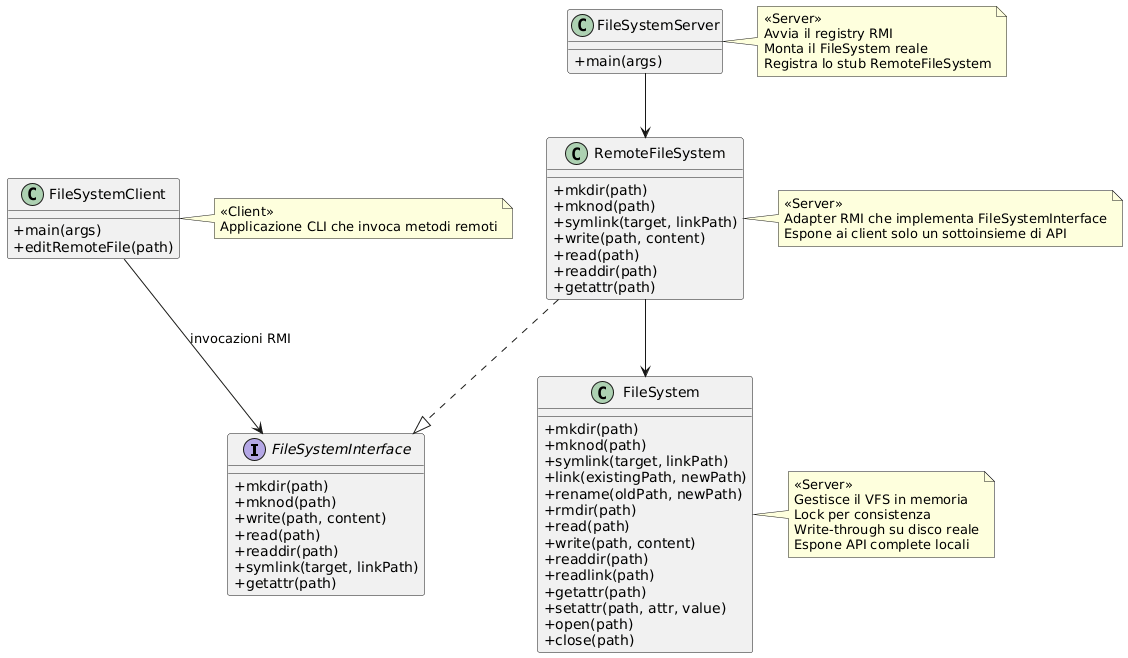
\includegraphics[keepaspectratio]{img/arch.png}}
\caption{Architettura client-server DVFS}
\end{figure}
\newpage
\section{Consistenza}\label{consistenza}

La consistenza è garantita dal \textbf{file system}. Ogni operazione che
modifica lo stato (scrittura, rinomina, rimozione) viene protetta da
lock a livello di path (\textbf{ReentrantReadWriteLock}).

\begin{itemize}
\tightlist
\item
  Più client possono leggere contemporaneamente senza conflitti.
\item
  Le scritture sono serializzate, impedendo \textbf{race condition}.
\item
  Ogni modifica avviene in due fasi: aggiornamento in memoria e
  write-through su disco.
\end{itemize}

I client non gestiscono lock: tutta la concorrenza viene risolta dal
server, che possiede l'unica copia ``autorevole'' dello stato.

\section{Montaggio da directory
reale}\label{montaggio-da-directory-reale}

Il sistema può partire da zero o essere montato da una directory
esistente. In questo caso, il contenuto viene caricato ricorsivamente:

\begin{itemize}
\tightlist
\item
  Directory → DirectoryNode.
\item
  File → FileNode (contenuto letto in memoria).
\item
  Symlink → SymlinkNode (target salvato).
\end{itemize}

La root del VFS viene rinominata ``/'', e ogni operazione successiva
(scrittura, rinomina, rimozione) viene riflessa anche sulla directory
reale tramite write-through.

\section{Funzionalità}\label{funzionalituxe0}

Il DVFS mette a disposizione un set completo di operazioni:

\begin{itemize}
\tightlist
\item
  \textbf{Creazione}: mkdir, mknod, symlink, link.
\item
  \textbf{Navigazione}: lookup, readdir, readlink.
\item
  \textbf{Manipolazione}: read, write, rename, rmdir.
\item
  \textbf{Gestione attributi}: getattr, setattr.
\item
  \textbf{Gestione apertura/chiusura}: open, close.
\end{itemize}

Inoltre, lato client è disponibile il comando \textbf{edit}, che
consente di modificare un file remoto con un editor locale in maniera
trasparente.

\section{Protocolli}\label{protocolli}

La comunicazione tra client e server avviene tramite \textbf{Java RMI}.
Le invocazioni remote sono trasparenti: il client invoca metodi
sull'interfaccia \textbf{FileSystemInterface}, che vengono eseguiti dal
server sul VFS locale.

\subsection{Flusso tipico di
un'operazione}\label{flusso-tipico-di-unoperazione}

\begin{enumerate}
\tightlist
\item
  Il client invia una richiesta remota (es.
  \texttt{write("/foo",\ data)}).
\item
  Lo stub RMI inoltra la chiamata a RemoteFileSystem sul server.
\item
  RemoteFileSystem chiama il metodo corrispondente di FileSystem.
\item
  FileSystem acquisisce il lock, aggiorna lo stato in memoria e riflette
  la modifica su disco.
\item
  Il risultato viene restituito al client.
\end{enumerate}

\begin{figure}
\centering
\pandocbounded{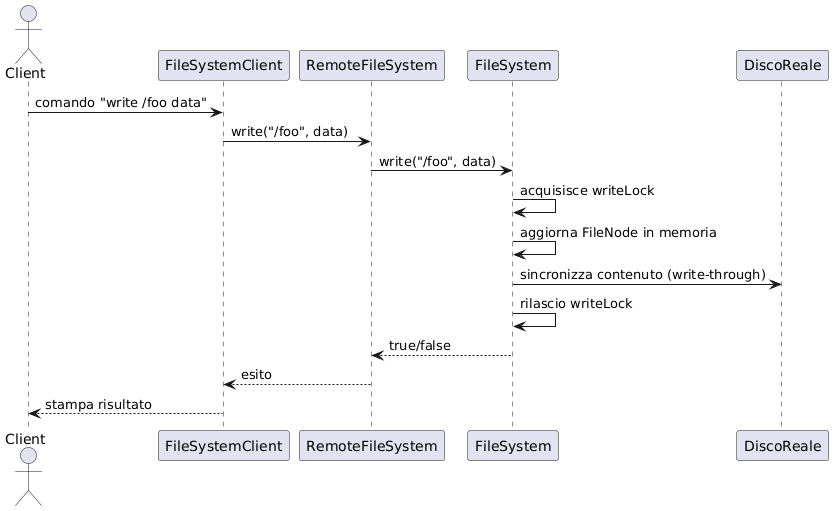
\includegraphics[keepaspectratio]{img/uml_op.png}}
\caption{Flusso di una richiesta write}
\end{figure}

\section{Sicurezza ed error handling}\label{sicurezza-ed-error-handling}

\begin{itemize}
\tightlist
\item
  Durante la risoluzione dei path, il server impedisce accessi fuori
  dalla root montata (protezione da path traversal).
\item
  In caso di errori I/O durante il write-through, l'operazione resta
  valida in memoria, evitando perdita di dati.
\item
  Gli errori lato server vengono propagati al client come eccezioni RMI.
\end{itemize}


\end{document}
